%%%%%%%%%%%%%%%%%%%%%%%%%%%%%%%%%%%%%%%%%
% Programming/Coding Assignment
% LaTeX Template
%
% This template has been downloaded from:
% http://www.latextemplates.com
%
% Original author:
% Ted Pavlic (http://www.tedpavlic.com)
%
% Note:
% The \lipsum[#] commands throughout this template generate dummy text
% to fill the template out. These commands should all be removed when
% writing assignment content.
%
% This template uses a Perl script as an example snippet of code, most other
% languages are also usable. Configure them in the "CODE INCLUSION
% CONFIGURATION" section.
%
%%%%%%%%%%%%%%%%%%%%%%%%%%%%%%%%%%%%%%%%%

%----------------------------------------------------------------------------------------
% PACKAGES AND OTHER DOCUMENT CONFIGURATIONS
%----------------------------------------------------------------------------------------

\documentclass{scrartcl}

\usepackage[T1]{fontenc}
\usepackage[utf8x]{inputenc}

\usepackage{fancyhdr} % Required for custom headers
\usepackage{lastpage} % Required to determine the last page for the footer
\usepackage{extramarks} % Required for headers and footers
\usepackage[usenames,dvipsnames]{color} % Required for custom colors
\usepackage{graphicx} % Required to insert images
\usepackage{listings} % Required for insertion of code
\usepackage{courier} % Required for the courier font

\usepackage{hyperref}

\linespread{1.1} % Line spacing

% Set up the header and footer
\pagestyle{fancy}
\lhead{\hmwkAuthorName \\} % Top left header
\chead{\hmwkClass: \hmwkTitle} % Top center head
\rhead{\firstxmark} % Top right header
\lfoot{\lastxmark} % Bottom left footer
\cfoot{} % Bottom center footer
\rfoot{Page\ \thepage\ of\ \protect\pageref{LastPage}} % Bottom right footer
\renewcommand\headrulewidth{0.4pt} % Size of the header rule
\renewcommand\footrulewidth{0.4pt} % Size of the footer rule

\setlength\parindent{0pt} % Removes all indentation from paragraphs

%----------------------------------------------------------------------------------------
%	CODE LISTINGS SETUP
%----------------------------------------------------------------------------------------
\usepackage{color}
\usepackage[usenames,dvipsnames,svgnames,table]{xcolor}
\colorlet{MAROON}{Maroon}
\usepackage{minted}
\providecommand*{\listingautorefname}{Listing}

%----------------------------------------------------------------------------------------
% NAME AND CLASS SECTION
%----------------------------------------------------------------------------------------

\newcommand{\hmwkTitle}{Project 2 -- Building a General Constraint-Based Puzzle Solver} % Assignment title
\newcommand{\hmwkDueDate}{Wednesday,\ October\ 24,\ 2013} % Due date
\newcommand{\hmwkClass}{IT3105} % Course/class
\newcommand{\hmwkClassTime}{} % Class/lecture time
\newcommand{\hmwkClassInstructor}{Lecturer: Keith Downing} % Teacher/lecturer
\newcommand{\hmwkAuthorName}{Pablo Liste Garcia \& Dominik Horb} % Your name

%----------------------------------------------------------------------------------------
% TITLE PAGE
%----------------------------------------------------------------------------------------

\title{
\vspace{2in}
\textmd{\textbf{\hmwkClass:\ \hmwkTitle}}\\
\normalsize\vspace{0.1in}\small{Due\ on\ \hmwkDueDate}\\
\vspace{0.1in}\large{\textit{\hmwkClassInstructor\ \hmwkClassTime}}
\vspace{3in}
}

\author{\textbf{\hmwkAuthorName}}
\date{} % Insert date here if you want it to appear below your name

%----------------------------------------------------------------------------------------

\begin{document}

\maketitle

%----------------------------------------------------------------------------------------
% TABLE OF CONTENTS
%----------------------------------------------------------------------------------------

%\setcounter{tocdepth}{1} % Uncomment this line if you don't want subsections listed in the ToC

\newpage
\tableofcontents
\newpage

\section{Architecture Description}

The general structure we chose to use for our implementation of the general puzzle solver doesn't deviate much from the proposed architecture in the task description. \autoref{fig:architecture} shows the two most important packages we created and their contained types. As you can see the main additions we made are \textit{PuzzleState}, \textit{Conflict} and \textit{GeneralPuzzleSolver}.

Our main class that creates the state manager and algorithm objects, initiates the execution and calculates the statistics is \textit{GeneralPuzzleSolver}. It could probably be refactored to separate the different tasks it has a bit more cleanly and distribute the problem specific initialization steps, but this is trivially achievable and wasn't a priority for now. To start an algorithm it creates an object of the desired \textit{LocalStateManager} for the puzzle that should be solved, provides it to an object of the chosen algorithm and starts the algorithm as can be seen in \autoref{lst:starting}.

\begin{listing}[H]
\caption{Combining algorithm and puzzle and starting the search.}
\label{lst:starting}
\begin{minted}[linenos=true]{java}
this.puzzle = this.choosePuzzle();
this.searcher = this.chooseSearchAlgorithm();
this.searcher.setStateManager(this.puzzle);
    
this.numberOfRuns = this.chooseNumberOfRuns();

PuzzleState currentSolution;

for (int i = 0; i < this.numberOfRuns; i++) {
  currentSolution = this.searcher.run();
  currentSolution.display();
}
\end{minted}
\end{listing}

 \begin{figure}[!htbp]
 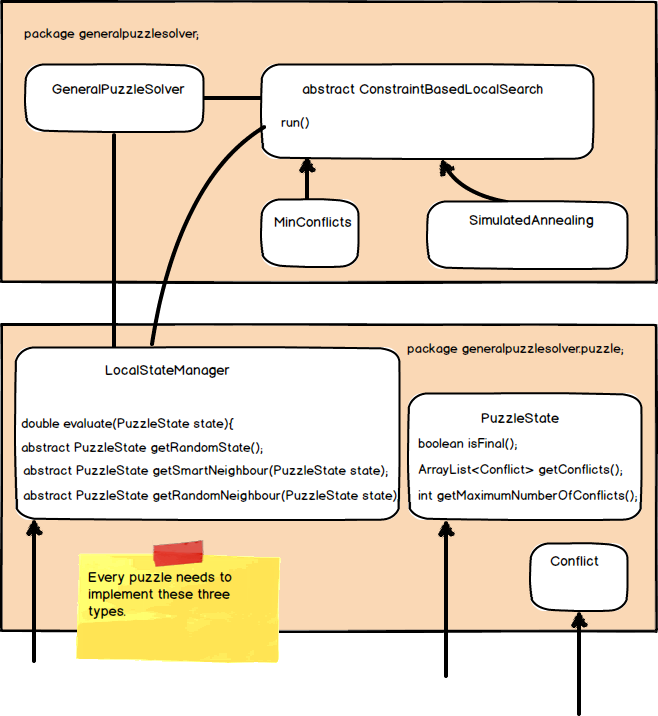
\includegraphics[width=1.0\linewidth]{graphics/architecture-diagram.png}
\caption{Architecture of our general puzzle solver.}\label{fig:architecture}
 \end{figure}

The more important bits can be found in the \textit{generalpuzzlesolver.puzzle} package. All three types that can be seen in the lower part of \autoref{fig:architecture} must be implemented by every puzzle that should be added to the application. The algorithm classes will only interact with methods that can be found within theses three types in order to generalize their execution.

\textit{Conflict} is simply an interface without any methods, but necessary to pass around specific conflicts. For the graph colouring problem an implementation would for example store the indices of two nodes that have the same colour and an edge in the graph.

As the name suggests, an implementation of \textit{PuzzleState} would simply store the data of the current state of the puzzle. It also needs to be able to check if it violates any constraints of the puzzle, provide a list of all the conflicts that exist and display itself.

To provide an example: In case of the graph colouring problem, it contains an adjacency matrix and a list with the data for all the vertices (colour and position).

The \textit{PuzzleStateManager} will be a stateless object in most cases, that just takes \textit{PuzzleState} objects into it's methods and changes them to some kind of ruleset provided inside the method.



\section{Third Puzzle: Sudoku}






\end{document}
